\subsubsection{Diodo led}


\begin{table}[H]
\begin{center}
\begin{tabular}{|c|c|c c c c c c c c c|}
    \hline
    unit & +/- \% & \multicolumn{9}{c|}{Osservazioni}\\ 
    \hline
    V & 0.01 & 1.85 & 2.20 & 2.25 & 2.30 & 2.35 & 2.40 & 2.45 & 2.50 & 2.55 \\ 
    mA & 1 & 0.01 & 0.01 & 0.01 & 0.02 & 0.06 & 0.15 & 0.33 & 0.54 & 0.88 \\ 
    \hline
    V & 0.01 & 2.60 & 2.65 & 2.70 & 2.75 & 2.80 & 2.85 & 2.90 & 2.95 & 3.00 \\ 
    mA & 1 & 1.32 & 1.93 & 2.54 & 3.33 & 4.11 & 5.08 & 6.02 & 7.45 & 8.45 \\ \hline
    \end{tabular}
    \end{center}
    \caption{Diodo led. Risposta corrente [mA] per tensione [V].}
    \label{C1_P3_dati}
\end{table}


Il grafico è stato fittato solo a partire da $V = 2.4 V$, ossia da dove parte la curvatura caratteristica.\\
La formula del fit è
$$ I = I_0 \cdot (e^{qV/gkt} -1) + a\cdot V $$
Il termine $a$ indica che si è tenuto conto del fatto che il diodo è led, e quindi si comporta come se avesse in parallelo una resistenza).\\
$  \frac{q}{kt} \approx 38.6 $ e $g$ è una costante adimensionale caratteristica del diodo.

\begin{figure}[H]
\centering
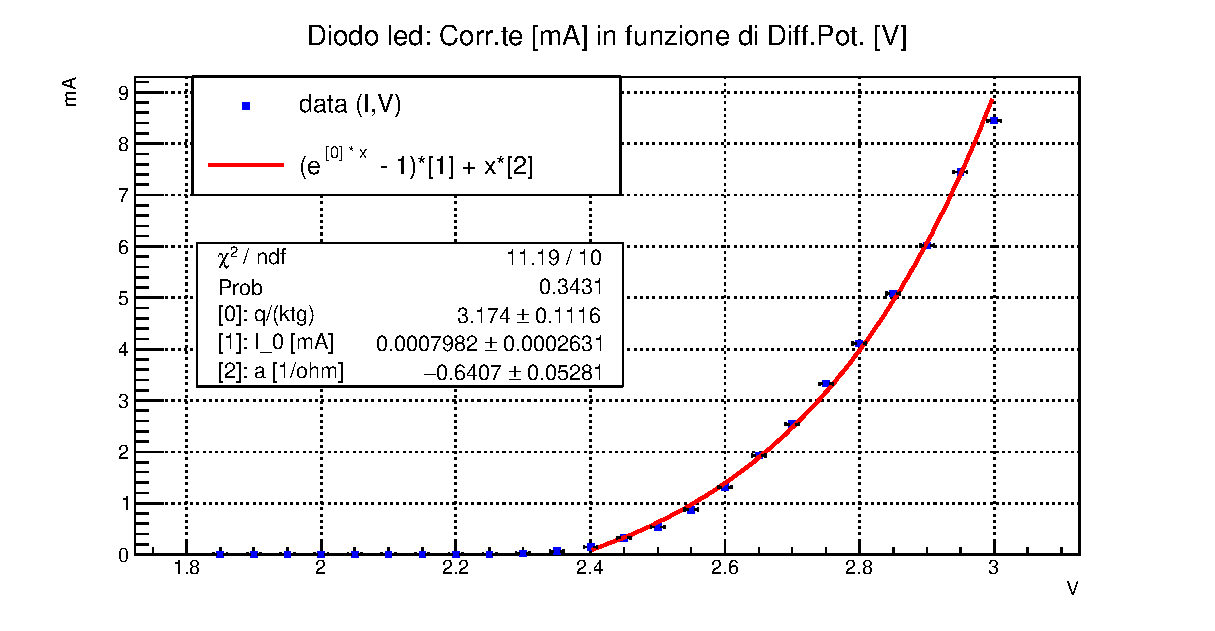
\includegraphics[scale=.7]{Grafici/C1_P3.eps}
\caption{
Risposta diodo led
}
\label{fig:C1_P3}
\end{figure}
%
%
Il chi quadro ridotto è molto vicino a 1, il che indica un buon adattamento dei dati al fit.